\section{Strategies, Details and Statistics}
\label{secStrategies}

In this section, we describe the main strategies of our team (Sec.~\ref{sec:teamStrategies}) and we highlight the main results that we got (Sec.~\ref{sec:comparisonOtherTeams}).

\subsection{Team Strategies}
\label{sec:teamStrategies}

The strategy of the team has two moments. In the former, the agents explore the map to obtain achievement points and to define good zones as soon as possible. Thus, it is possible to get a good score in the first steps. In the latter, the agents start to conquer and protect several small zones. During the whole match, the saboteurs disturb the enemy and the repairers help disabled agents.


\begin{figure}[th]
 \vspace{-5mm}
 \centering
 \subfigure[Hill]{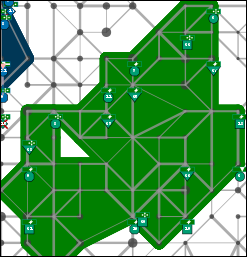
\includegraphics[width=0.4\textwidth]{figs/hill.png}\label{fig:hill}}
 \subfigure[Pivots]{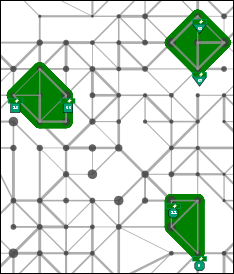
\includegraphics[width=0.3\textwidth]{figs/pivots.png}\label{fig:pivots}}
 \subfigure[Islands]{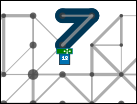
\includegraphics[width=0.17\textwidth]{figs/islands.png}\label{fig:islands}}
 \vspace{-3mm}\caption{Hills, pivots, and islands}
 \label{fig:hillislandpivot}
 \vspace{-3mm}
\end{figure}

The good zones are defined in terms of \emph{hills}, \emph{pivots}, and \emph{islands}. A hill (the big zone in Fig.~\ref{fig:hill}) is a zone formed by several vertices that have a good value and are in the same region of the map. As in the 2012 team, the agents try to discover two hills. The hills are defined as follows: for each vertex $v$ of the graph, the algorithm sums the values of all vertices up to two hops away from $v$, including $v$. The two vertices with the highest sums are defined as the center of the hills, and then the agents try to stay on the neighborhoods. The agents control the hills simply moving to the border of the hills in order to expand them. If they break the zone, they come back to the previous places and try to expand again. We also defined that the sentinels need to conquer the best vertices in the hills and stay over them all the time until the strategy changes. Sometimes, it induces the opponents to avoid those places and we guarantee a fixed gain of scores of the hills, even if the enemy is disturbing. Moreover, the explorers of the group \emph{special exploration} prefer to probe first the vertices in the hills, because it increases the gain of points in the first steps.


\begin{figure}[th]
 \vspace{-5mm}
 \centering
 \subfigure[]{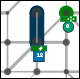
\includegraphics[width=0.15\textwidth, height=0.15\textwidth]{figs/protectIsland1.png}\label{fig:protectIsland1}}
 \subfigure[]{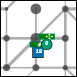
\includegraphics[width=0.15\textwidth, height=0.15\textwidth]{figs/protectIsland2.png}\label{fig:protectIsland2}}
 \subfigure[]{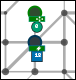
\includegraphics[width=0.15\textwidth, height=0.15\textwidth]{figs/protectIsland3.png}\label{fig:protectIsland3}}
 \subfigure[]{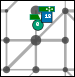
\includegraphics[width=0.15\textwidth, height=0.15\textwidth]{figs/protectIsland4.png}\label{fig:protectIsland4}}
 
 \vspace{-3mm}
 
 \subfigure[]{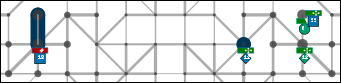
\includegraphics[width=0.65\textwidth]{figs/protectIsland5.png}\label{fig:protectIsland5}}
 \vspace{-3mm}\caption{Protecting islands}
 \label{fig:protectIslands}
 \vspace{-3mm}
\end{figure}

Islands (Fig.~\ref{fig:islands}) are regions of the map that can be conquered by a single agent. An island is a zone that has only one vertex (a \emph{cut vertex}) in common with the remaining graph. They are found by disconnecting the edges of each cut vertex of the graph. It produces two disconnected subgraphs, and the smallest one, plus the cut vertex, are an island. If there are enemies on the island, the controller agent will go to the same vertex of the enemy. Thus, both teams do not get the points of that island. The figures~\ref{fig:protectIsland1}, ~\ref{fig:protectIsland2},~\ref{fig:protectIsland3}, and~\ref{fig:protectIsland4} illustrate this situation. In addition, the controller agent notifies the saboteur leader about the invader. If the saboteur leader is already busy protecting another island, the saboteur leader calls the saboteur helper of the group \emph{special operations}. If both are busy the saboteur leader keeps a list of islands with enemies for a further attack. Fig.~\ref{fig:protectIsland5} illustrates a probable call of the saboteur leader (the diamond not at the cut vertex) that is going to fight against an explorer (the circle) and a saboteur (the diamond at the cut vertex).

Pivots (Fig.~\ref{fig:pivots}) are regions of the map that can be conquered by just two agents. For each pair of vertices ($u$,$v$) we search all vertices $w$ connected to $u$ and $v$. For all vertices $w$ (including $u$ and $v$) we also search all vertices only connected to these vertices. For example, if there is a vertice $k$ connected only to the vertice $w$, then $k$ also belongs to the pivot. Furthermore, if there is an island connected to some of these vertices we consider all the vertices of the island. The best pivots are chosen considering the sum of all vertices. The agents that control pivots do not move away from their places, since most of the time the enemy does not stay fixed in those places. However, if the enemy stays in the same vertex both teams do not get the points, and so our team also cancels the enemy strategy. This is another reason to not leave the vertices. Otherwise the opponent will get the points.

The hills are defined in the first phase of our strategy, until around step 130. We chose to use hills instead of islands and pivots in the beginning of the match because most of the vertices are still unprobed and so we would not get so many points. The use of hills can keep all agents together and getting higher points because the zones are bigger. After a while the agents start conquering pivots and islands. The agents also need to decide if it is better to conquer two islands or one pivot. The decision is taken by simply summing the value of two islands and comparing with the pivots. If the two islands provide the same gain of the pivot or if they are more valuable, the agents will prefer to conquer two islands instead of conquering one pivot. The pivots and islands are very stable and so our agents are not disturbed by the enemy while our agents can disturb their zones since it is harder to protect a big zone than several small zones. 

\begin{table}[th]
\vspace{-5mm}
\begin{center}

	\begin{tabular}{l c c c c c}
		\toprule
		Action & Repairer & Saboteur & Explorer & Sentinel & Inspector \\
		\midrule
		%\midrule
		attack &  & x &  &  &  \\
		%\midrule
		repair & x &  &  &  &  \\
		%\midrule
		parry & x &  &  & x &  \\
		%\midrule
		probe &  &  & x &  &  \\
		%\midrule
		inspect &  &  &  &  & x \\
		%\midrule
		recharge & x & x & x & x & x \\
		%\midrule
		goto & x & x & x & x & x \\
		%\midrule
		survey & x & x & x & x & x \\
		\bottomrule            
                
	\end{tabular}
\end{center}
\caption{Implemented strategies by agent type. \label{tab:tabStrategies}}
\vspace{-5mm}
\end{table}

The achievements continue to be as important as in the last year. We decided do not waste money buying items and get as much achievements as possible and as soon as possible, since they accumulate in each step. We made this decision since in our tests we did not see any advantage in buying items. Finally, the specific strategies of each kind of agent are explained below while Table~\ref{tab:tabStrategies} summarizes the strategies implemented for each kind of agent.

\vspace{-3mm}

\begin{description}
 \item[Explorer:] the explorers have an important role in the beginning of the match. They need to probe all vertices as soon as possible. To do so, the explorers avoid performing the survey action and conquering zones until they have probed all vertices. Furthermore, the \emph{explorer leader} defines the initial two hills.
 \item[Saboteur:] the main aims of the saboteurs are to protect the islands and disturb the enemy. The saboteur with the role \emph{saboteur chaser} has the aim to attack mainly explorers, inspectors, sentinels, and repairers to avoid staying in the same vertex fighting against saboteurs all the time. The saboteurs with the roles \emph{saboteur leader} and \emph{saboteur helper} have the main aim to protect islands against enemies. The \emph{saboteur leader} is also the main contact of the other agents to ask for help. In other cases, the saboteurs simply search and destroy enemies. In addition, the saboteurs attack following a priority. First of all they prefer to attack saboteurs, followed by explorers, inspectors, repairers, and sentinels. The saboteurs prefer to attack explorers and inspectors because they can not parry.
 \item[Repairer:] the main aim of the repairers is to keep the agents enabled. All agents that are disabled inform the \emph{repairer leader}. The \emph{repairer leader} asks all the other repairers if they can help the disabled agents. If a repairer is not committed to an agent and it is not getting high points and it is enabled, then it is apt to help the other agent. All apt repairers inform the path size until the disabled agent and the \emph{repairer leader} chooses the closest repairer to help the disabled agent. To make the repair operation faster, both the repairer agent and the disabled agent follow the same path to meet each other. If there is some repairer next to the disabled agent, that repairer will repair the agent and the agent will cancel the appointment with its repairer. Finally, when the repairers are not helping the disabled agents, they also go to the pivots or islands that they belong to.
 \item[Sentinel:] the sentinels always protect the best zones, since they are harder to get disabled and they can parry. They are usually avoided by the enemy because they do not have an important role like repairers, explorers, and saboteurs. Therefore, the sentinels are not disturbed so often. The sentinels also try to survey if they find some vertex with edges with unknown value. Finally, the \emph{sentinel leader} has the aim to define the islands and pivots and inform the agents about it.
 \item[Inspector:] the inspectors protect the next best zones, since they are also not so disturbed by the enemies. Their aim is to inspect all the enemy agents and they do it just once, since we do not care about what the enemy is buying. Doing so, the inspectors can stay in the same vertices until the end of the match, getting more points than by inspecting enemies.
\end{description}

\subsection{Comparison to Other Teams}
\label{sec:comparisonOtherTeams}

\begin{figure}[th]
 \vspace{-5mm}
 \centering
 \subfigure[Scores]{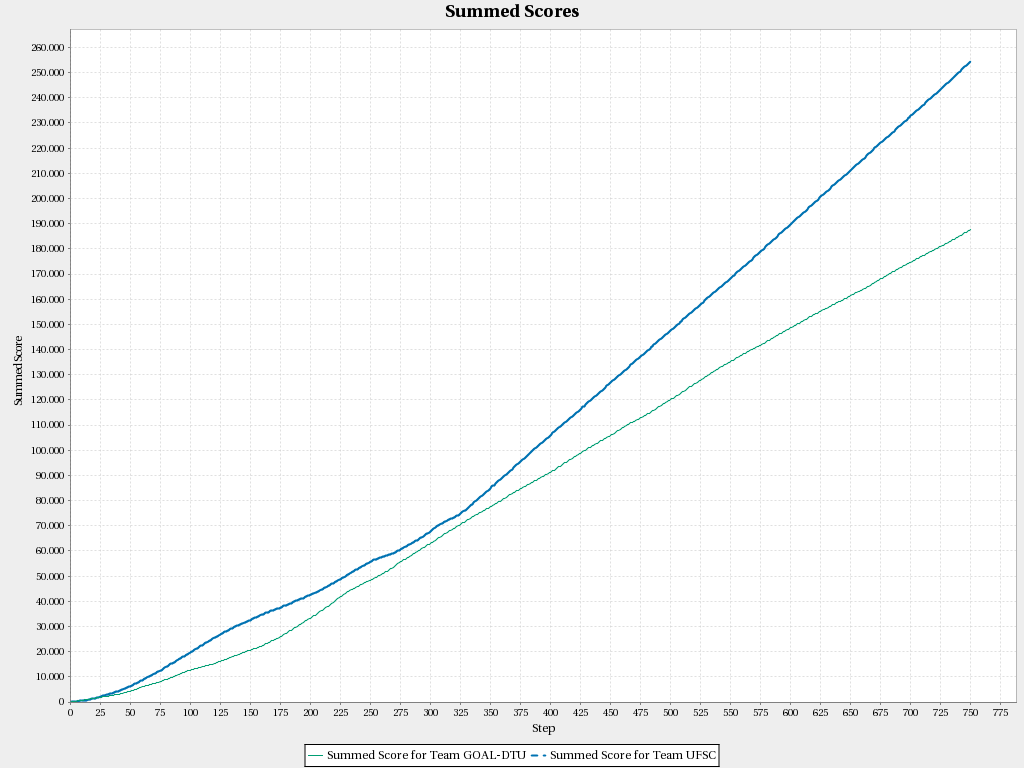
\includegraphics[width=0.49\textwidth]{figs/Scores.png}\label{fig:Scores}}
 \subfigure[ZoneStabilities]{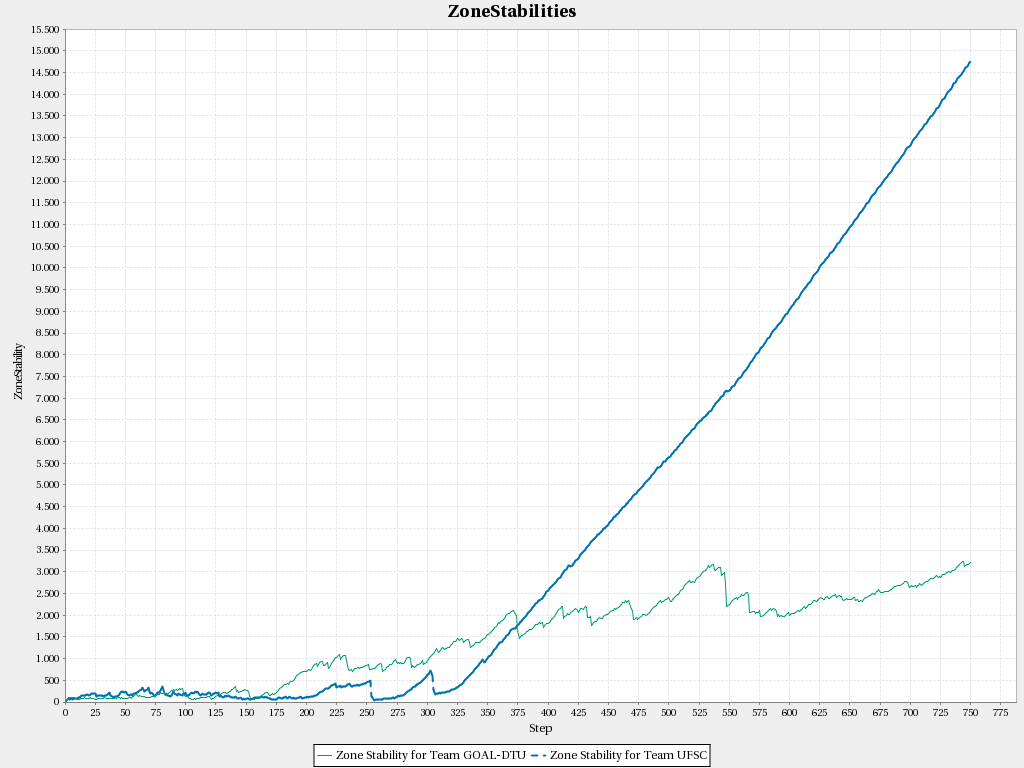
\includegraphics[width=0.49\textwidth]{figs/ZoneStabilities.png}\label{fig:ZoneStabilities}}
 
 \vspace{-3mm}
 
 \subfigure[AchievementPoints]{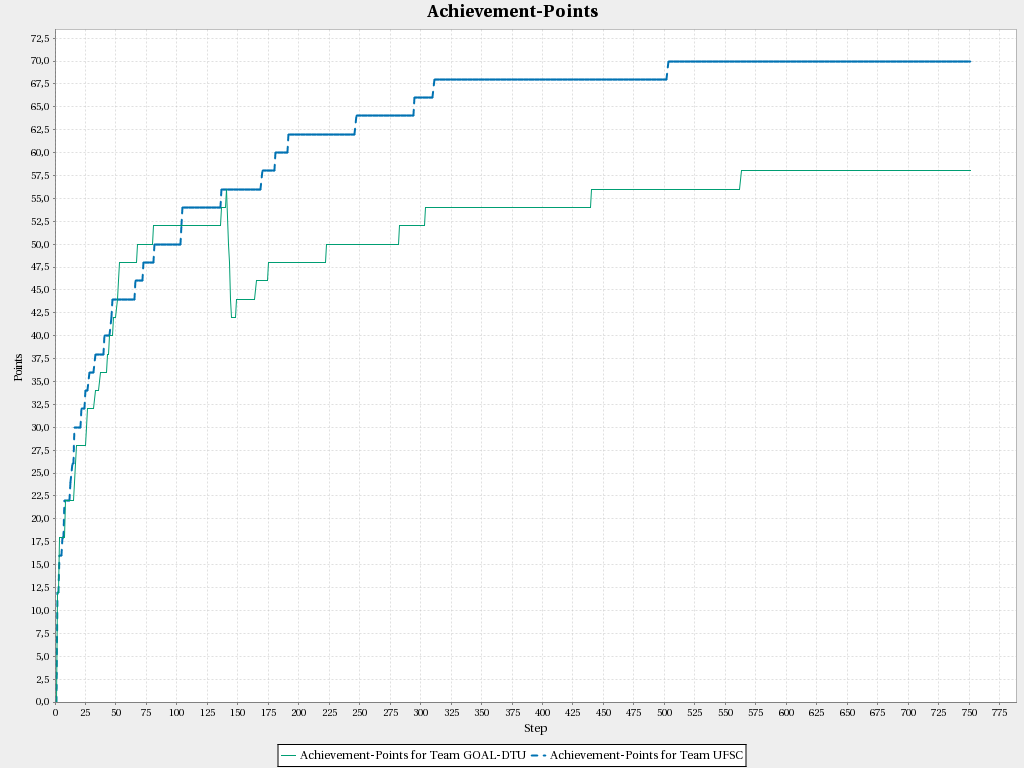
\includegraphics[width=0.49\textwidth]{figs/AchievementPoints.png}\label{fig:AchievementPoints}}
 \subfigure[ZonesScores]{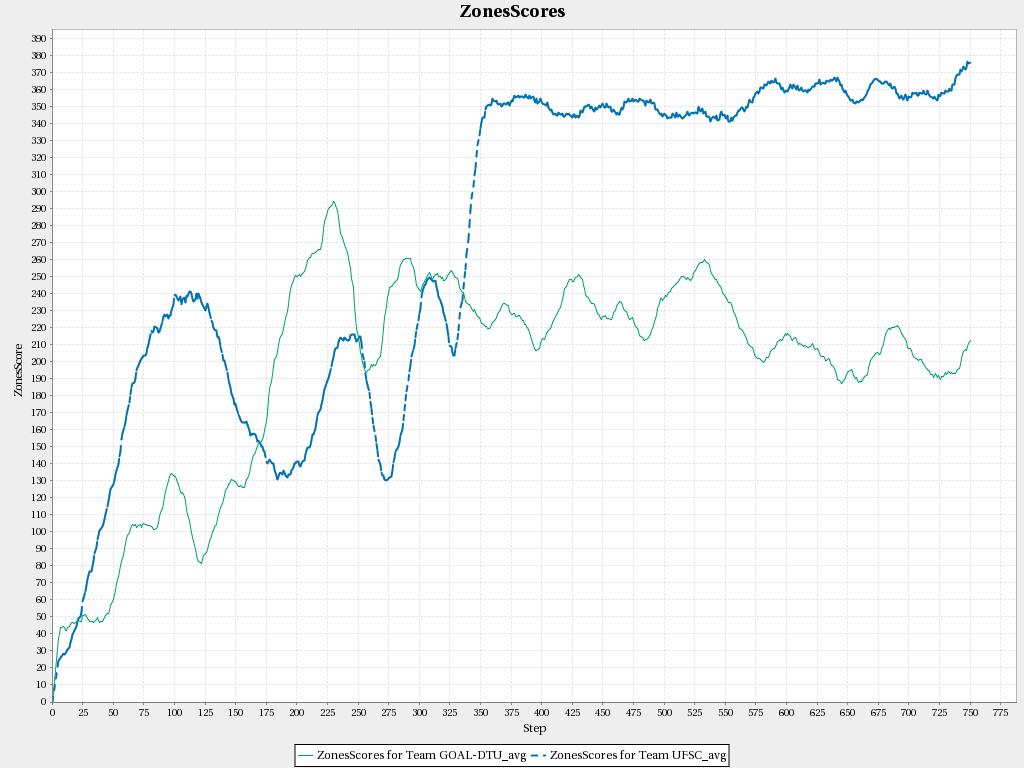
\includegraphics[width=0.49\textwidth]{figs/ZonesScores.png}\label{fig:ZonesScores}} 
 \vspace{-3mm}\caption{Statistics}
 \label{fig:statistics}
 \vspace{-3mm}
\end{figure}

In order to highlight the main results of our strategy we chose to use some statistics of the second match against the GOAL-DTU team \footnote{\url{http://multiagentcontest.org/downloads/func-startdown/1716/}}, which got the second place. Due our strategy of small zones, we can verify in the Fig.~\ref{fig:ZoneStabilities}  that after step 325 our team (blue) kept almost the same zones until the end of the match. This behavior is usual in all matches against the other teams. The reason is that no matter what the opponent does, our agents will rarely leave their positions.

Another interesting result can be drawn from the zones scores plot (Fig.~\ref{fig:ZonesScores}). We can see that our team (blue) kept getting almost the same zone scores after step 350 and always more than the opponent. The phase of hills can also be noticed in the beginning of the match, between step 25 until around step 130, where the team is getting high scores because of the big zones. After step 130 our team started to conquer small zones (pivots and islands) and, therefore, spreading the agents out over the whole map. It is also possible to see that, sometimes, our zone scores were lower than the enemies. This was an expected behavior when the agents were still changing their positions because the explorers were still probing new vertices. We can see it after step 250 and after around step 315, where our team decreased the gain of zone scores. After probing all vertices (around step 325), the agents started to get higher scores because they defined the fixed zones and all agents were participating.

We can see the same behavior in Fig.~\ref{fig:Scores}, where the opponent score gets closer and then the difference of scores increases again. Notice that after step 325 the difference of scores increased continuously because all vertices were probed. On the other hand, in the Fig.~\ref{fig:AchievementPoints} we can see that our team always has more achievement points than the opponent after step 125. It means we are getting more points because the opponent was buying items while our team was saving money.